% This must be in the first 5 lines to tell arXiv to use pdfLaTeX, which is strongly recommended.
\pdfoutput=1
% In particular, the hyperref package requires pdfLaTeX in order to break URLs across lines.

\documentclass[11pt]{article}


% Change "review" to "final" to generate the final (sometimes called camera-ready) version.
% Change to "preprint" to generate a non-anonymous version with page numbers.
% \usepackage[review]{acl}
\usepackage[final]{acl}

% Standard package includes
\usepackage{times}
\usepackage{latexsym}

% For proper rendering and hyphenation of words containing Latin characters (including in bib files)
\usepackage[T1]{fontenc}
% For Vietnamese characters
% \usepackage[T5]{fontenc}
% See https://www.latex-project.org/help/documentation/encguide.pdf for other character sets

% This assumes your files are encoded as UTF8
\usepackage[utf8]{inputenc}

% This is not strictly necessary, and may be commented out,
% but it will improve the layout of the manuscript,
% and will typically save some space.
\usepackage{microtype}

% This is also not strictly necessary, and may be commented out.
% However, it will improve the aesthetics of text in
% the typewriter font.
\usepackage{inconsolata}

%Including images in your LaTeX document requires adding
%additional package(s)
\usepackage{graphicx}

% If the title and author information does not fit in the area allocated, uncomment the following
%
%\setlength\titlebox{<dim>}
%
% and set <dim> to something 5cm or larger.


%%%%%%%%%%%%%%%%%%%%%%%%%%%%%%%%%%%%%%%%%%%%%%%%%%%%%%%%%%%%%%%
% OWN PACKAGES
%%%%%%%%%%%%%%%%%%%%%%%%%%%%%%%%%%%%%%%%%%%%%%%%%%%%%%%%%%%%%%%

\usepackage{url}

%
% Python code blocks
%
\usepackage{listings}
\usepackage{xcolor}
% Define colors for Python syntax highlighting
\definecolor{pystring}{rgb}{0.164, 0.631, 0.596}    % strings
\definecolor{pycomment}{rgb}{0.498, 0.498, 0.498}   % comments
\definecolor{pykeyword}{rgb}{0.737, 0.353, 0.662}   % keywords
\definecolor{pybackground}{rgb}{0.95, 0.95, 0.95}   % background
\definecolor{pyfunction}{rgb}{0.164, 0.631, 0.596}  % function names
% Configure Python listing style
\lstdefinestyle{pythonstyle}{
    language=Python,
    backgroundcolor=\color{pybackground},
    basicstyle=\ttfamily\footnotesize,
    breakatwhitespace=false,
    breaklines=true,
    captionpos=b,
    keepspaces=true,
    numbers=left,
    numbersep=5pt,
    showspaces=false,
    showstringspaces=false,
    showtabs=false,
    tabsize=4,
    frame=single,
    commentstyle=\color{pycomment},
    keywordstyle=\color{pykeyword},
    stringstyle=\color{pystring},
    numberstyle=\tiny\color{pycomment},
    identifierstyle=\color{black},
    emphstyle=\color{pyfunction}
}
% Set the defined style as default
\lstset{style=pythonstyle}


% Define commands for colored marks
\usepackage{xcolor}
\usepackage{pifont}
\usepackage{wasysym}
\newcommand{\cmark}{\textcolor{green}{\ding{51}}}
\newcommand{\xmark}{\textcolor{red}{\ding{55}}}
\newcommand{\pmark}{\textcolor{orange}{\Circle}}

%%%%%%%%%%%%%%%%%%%%%%%%%%%%%%%%%%%%%%%%%%%%%%%%%%%%%%%%%%%%%%%
% / OWN PACKAGES
%%%%%%%%%%%%%%%%%%%%%%%%%%%%%%%%%%%%%%%%%%%%%%%%%%%%%%%%%%%%%%%


\title{IGC: Integrating a Gated Calculator into an LLM to Solve Arithmetic Tasks Reliably and Efficiently}

% Author information can be set in various styles:
% For several authors from the same institution:
% \author{Author 1 \and ... \and Author n \\
%         Address line \\ ... \\ Address line}
% if the names do not fit well on one line use
%         Author 1 \\ {\bf Author 2} \\ ... \\ {\bf Author n} \\
% For authors from different institutions:
% \author{Author 1 \\ Address line \\  ... \\ Address line
%         \And  ... \And
%         Author n \\ Address line \\ ... \\ Address line}
% To start a separate ``row'' of authors use \AND, as in
% \author{Author 1 \\ Address line \\  ... \\ Address line
%         \AND
%         Author 2 \\ Address line \\ ... \\ Address line \And
%         Author 3 \\ Address line \\ ... \\ Address line}

\author{Florian Dietz \and Dietrich Klakow \\
  Spoken Language Systems (LSV), Saarland University, Saarbrücken, Germany \\
 \small{
   \textbf{Correspondence:} \href{mailto:fdietz@lsv.uni-saarland.de}{fdietz@lsv.uni-saarland.de}
 }
}

\begin{document}
\maketitle
\footnotetext{This paper is currently under review at ACL Rolling Review.}
\begin{abstract}


Solving arithmetic tasks is a simple and fundamental skill, yet modern Large Language Models (LLMs) have great difficulty with them.
We introduce the Integrated Gated Calculator (IGC), a module that enables LLMs to perform arithmetic by emulating a calculator on the GPU.
We finetune a Llama model with our module and test it on the BigBench Arithmetic benchmark, where it beats the State of the Art, outperforming all models on the benchmark, including models almost two orders of magnitude larger.
Our approach takes only a single iteration to run and requires no external tools. It performs arithmetic operations entirely inside the LLM without the need to produce intermediate tokens. It is computationally efficient, interpretable, and avoids side-effects on tasks that do not require arithmetic operations.
It reliably achieves 98\% to 99\% accuracy across multiple training runs and for all subtasks, including the substantially harder subtask of multiplication, which was previously unsolved.



\end{abstract}



\section{Introduction}



\textbf{Motivation}.
Large Language Models (LLM) have shown impressive abilities in many different fields in recent years \citep{thoppilan2022lamda,chowdhery2023palm,brown2020language}.
This makes it all the more intriguing that even advanced LLMs still perform very poorly on basic arithmetic tasks:
GPT-3 has trouble adding numbers with more than three digits \citep{brown2020language} and GPT-4 \citep{achiam2023gpt} still fails to solve multiplication tasks \citep{dziri2024faith}.
The reasons for this surprisingly poor performance have been studied extensively \citep{yuan2023well,brown2020language,dziri2024faith}.
Even so the BigBench Arithmetic benchmark \citep{srivastava2023beyond}, which tests the four basic arithmetic operations on merely 5-digit long numbers, remains unsolved.
% OPTIONAL
% Many techniques have been proposed to add arithmetic abilities to LLMs, but each of them either fails to generalize or has requirements that make it impractical.



\begin{figure}
    \centering
    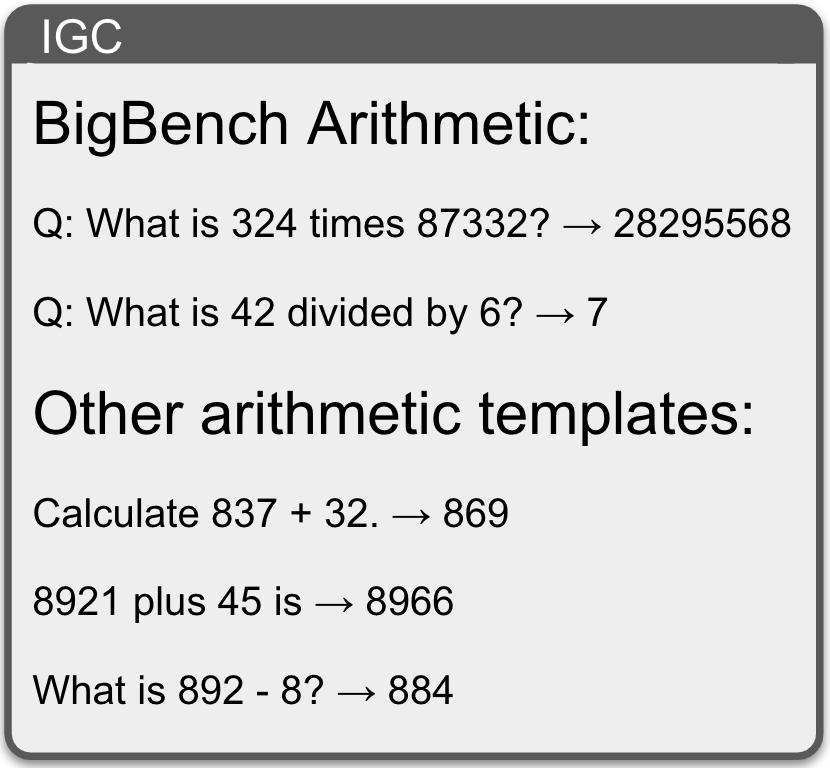
\includegraphics[width=0.7\linewidth]{images/templates.png}
    \caption{Examples of arithmetic tasks.
    % Unlike the benchmark, our training uses both text operators ("plus") and symbolic operators ("+").
    }
    \label{fig:training_templates}
\end{figure}

\textbf{The Impact of Number Representations}.
The arithmetic abilities of LLMs strongly depend on the way numbers are represented \citep{thawani2021representing}.
\citet{mcleish2024transformers} improve arithmetic performance by adding positional encodings to numbers.
% DUPLICATE - GOAT
Similarly, \citet{liu2023goatfinetunedllamaoutperforms} show that good performance can be achieved on addition and subtraction tasks using finetuning only, and they attribute this to the especially well-suited tokenization method of their model.
However, we are not aware of any finetuning method that solves the more difficult subtask of multiplication effectively.


% NH: This section seems duplicated in related work?
% --> I tried to mentioned strengths/weaknesses of COT and tool use in this section, and to give examples in related work. If I have a related work section at all, then it needs to be mentioned there. But I also want to mention it in the introduction because it's relevant to the decision why our method is needed.
\textbf{Chain of Thought}.
Chain of Thought (COT) is a prompting method that works by breaking the task down into smaller subtasks and solving them step-by-step \citep{wei2023chainofthoughtpromptingelicitsreasoning}.
This approach makes many difficult tasks solvable, but it also increases the model's runtime as it requires many intermediate outputs to produce the final result.


% NH: This section seems duplicated in related work?
\textbf{Tool Use}.
\citet{schick2023toolformerlanguagemodelsteach} introduced the Toolformer, which teaches LLMs to call external tools.
This method is very powerful, but it increases the inference time due to costly transfers of data between the GPU and CPU.
% OPTIONAL I am also mentioning this later
Moreover, since this method is only added after pretraining, the LLM can't learn to condition its predictions on the results of arithmetic operations during pretraining.
Since arithmetic is a fundamental building block of more complex tasks, it would be worthwhile to enable LLMs to solve arithmetic tasks directly during pretraining, so that it can use this ability as a subroutine for more complex problems.


\textbf{Our Solution}.
We develop the \textit{Integrated Gated Calculator} (IGC), a module that enables an LLM to accurately perform arithmetic operations, in a single iteration and without using external tools.
It extracts numbers from the tokens in a categorical representation and then emulates the calculation directly on the GPU.
% OPTIONAL - some of this is redundant, it can be shortened
% Our approach is efficiently trainable and uses a negligible number of parameters. The calculator emulation is provably perfect and only the mappings between tokens and calculator need to be learned.
% The approach works even for models whose tokenization uses a suboptimal number representation.
% Finally, its use of gates with learned weights allow it to be integrated into an LLM with minimal impact on other tasks, reducing the risk of destructive interference.


Our contributions are:

\begin{itemize}
    \item \textbf{Innovation}.
    We introduce the \textit{Integrated Gated Calculator}, a novel module that can emulate a calculator (Section~\ref{section-methods}).
    We modify a pretrained Llama 3.1 8B model \citep{touvron2023llama,dubey2024llama} with it and finetune on synthetic data. This enables the LLM to solve complex arithmetic tasks reliably, directly on the GPU, without using COTs, a scratchpad, or calling any tools.
    \item \textbf{Results}.
    We achieve near-perfect generalization on the BigBench Arithmetic Benchmark, outperforming SOTA models that are almost two orders of magnitude larger (Section~\ref{section-experiments}).
    To the best of our knowledge, we are the first to enable an LLM to solve multiplication tasks without the use of external tools or lengthy multi-step procedures.
    \item \textbf{Analysis}.
    We compare our approach with alternatives (Section~\ref{section-comparison-of-methods}) and find that it has numerous advantages besides its strong performance on the benchmark: It is both computationally efficient and interpretable, and it can learn to avoid side effects and destructive interference for problems that do not require arithmetics.
    \item \textbf{Future Work}.
    % Practical applications
    We describe how the IGC could be integrated into an LLM during pretraining instead of finetuning (Section~\ref{section-future-work}). This would allow the LLM to learn to use it as a subroutine for more complex tasks, an ability that is missing from alternative approaches.
    % Extensions
    We further describe how our approach could be generalized and extended to other non-differentiable operations, such as looking up items in a database.
\end{itemize}



\section{Related Work}



% OPTIONAL - shorten this? In extreme cases, this could be dropped. But it's better to keep it because I reference the difference between arithmetic and word problems later and it's best if I have one central location where everything is defined.
\textbf{Word Problems}.
We want to highlight the fact that arithmetic tasks are different from math word problems.
In some cases, models fail to solve word problems even though they follow correct reasoning, because they get the arithmetic operations wrong \citep{schick2023toolformerlanguagemodelsteach,cobbe2021gsm8k,gao2023pal}.
In other cases, models fail to solve word problems with trivial arithmetic operations because they fail to extract the numbers or to format the output correctly. We see examples of this in our analysis of existing benchmark data in Section~\ref{section-experiments}.
In this paper we focus on arithmetic. We discuss in Future Work (Section~\ref{section-future-work}) how our method could be integrated into an LLM more effectively than alternative approaches, which should help greatly with word problems, too.


% Keep this SHORT. It's not actually related, because my technique is different.
\textbf{Chain of Thought}.
Chain of Thought methods have shown promising results on a variety of different tasks and for many different models \citep{nye2021show,chung2024scaling}.
\citet{lee2023teachingarithmeticsmalltransformers} investigated ways to teach arithmetic to small transformers and found that COT can help significantly on this task as well.


% Keep this SHORT. It's not actually related, because my technique is different.
\textbf{Tool Use}.
\citet{schick2023toolformerlanguagemodelsteach} introduced the Toolformer, a generic method to enable an LLM to interact with an external tool. By interacting with a calculator, this method can perfectly solve arithmetic tasks of any complexity.
Tool use is a very generic technique with applications for many different tasks and domains \citep{qu2024tool}.


\textbf{Other Approaches for Arithmetic Tasks}.
\citet{cobbe2021gsm8k} train verifiers to solve math word problems.
\citet{nye2021show} add scratchpads to the COT approach.
\citet{imani2023mathpromptermathematicalreasoningusing} compares several Chains of Thoughts to improve reliability.
\citet{chen2022program} and \citet{gao2023pal} combine COT and Tool Use by generating executable code.


\textbf{Modifying LLMs}.
% TODO OPTIONAL maybe revert this change? Either give a list of methods or at least explicitly say it's too many to list and to look at this survey instead.
% NH: I actually like this paragraph :) but maybe make the forward-reference more precise? Or just say "the next section" --> done.
Many different techniques for modifying and finetuning LLMs exist \citet{ding2022delta}.
Our approach is most similar to Adapter-based methods \citep{houlsby2019parameter}, which work by injecting a separate smaller neural network into a pretrained LLM. This Adapter module is trained to modify one of the intermediate activations of the LLM, while the base LLM's parameters are kept frozen.
However, our method has several important differences to typical Adapter methods, which we explain in the next Section.%in Section~\ref{section-methods}.



\section{Methods}
\label{section-methods}


\begin{figure*}[t]
    \centering
    \frame{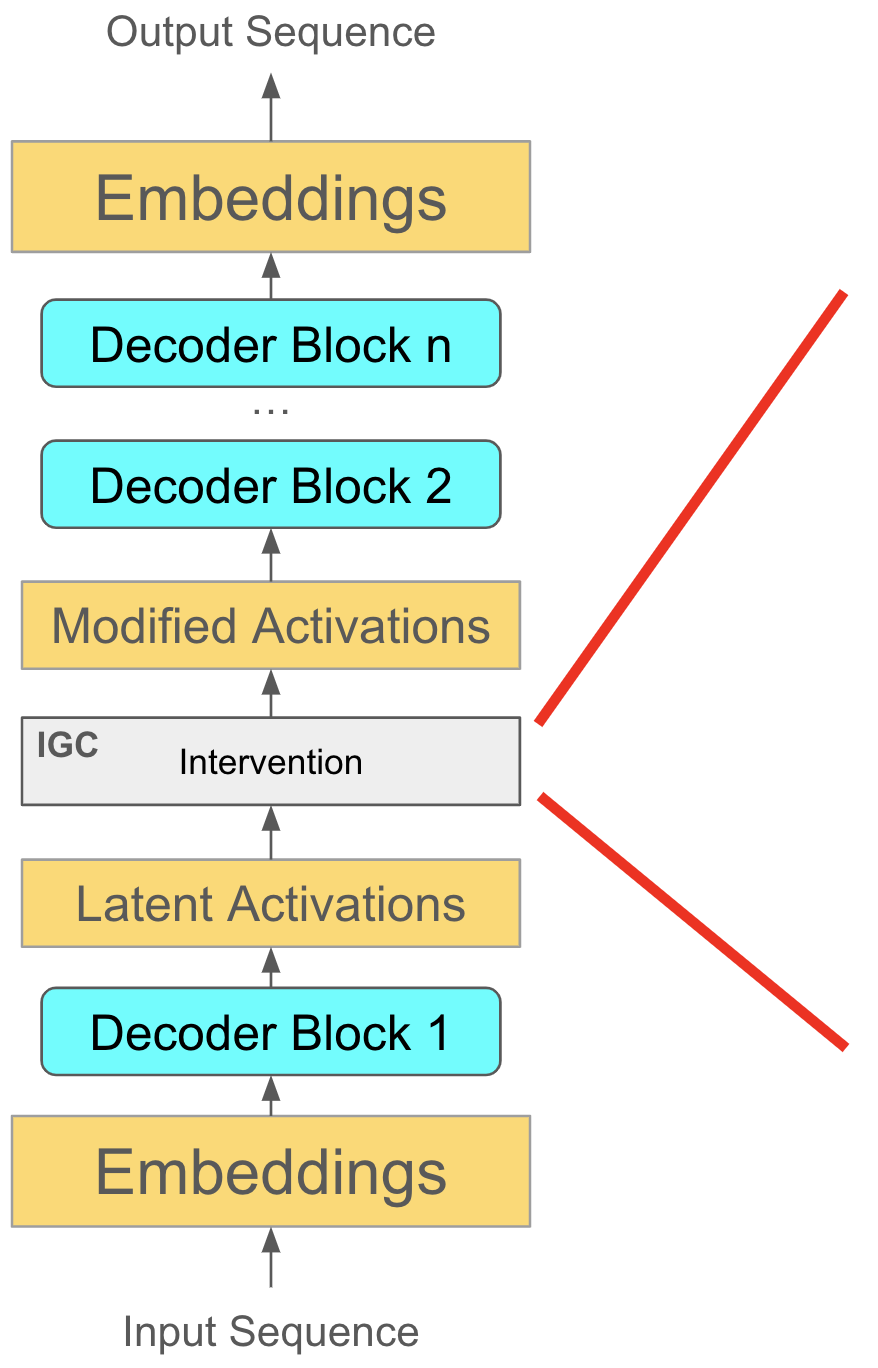
\includegraphics[width=0.279\linewidth]{images/architecture-placement.png}}
    \frame{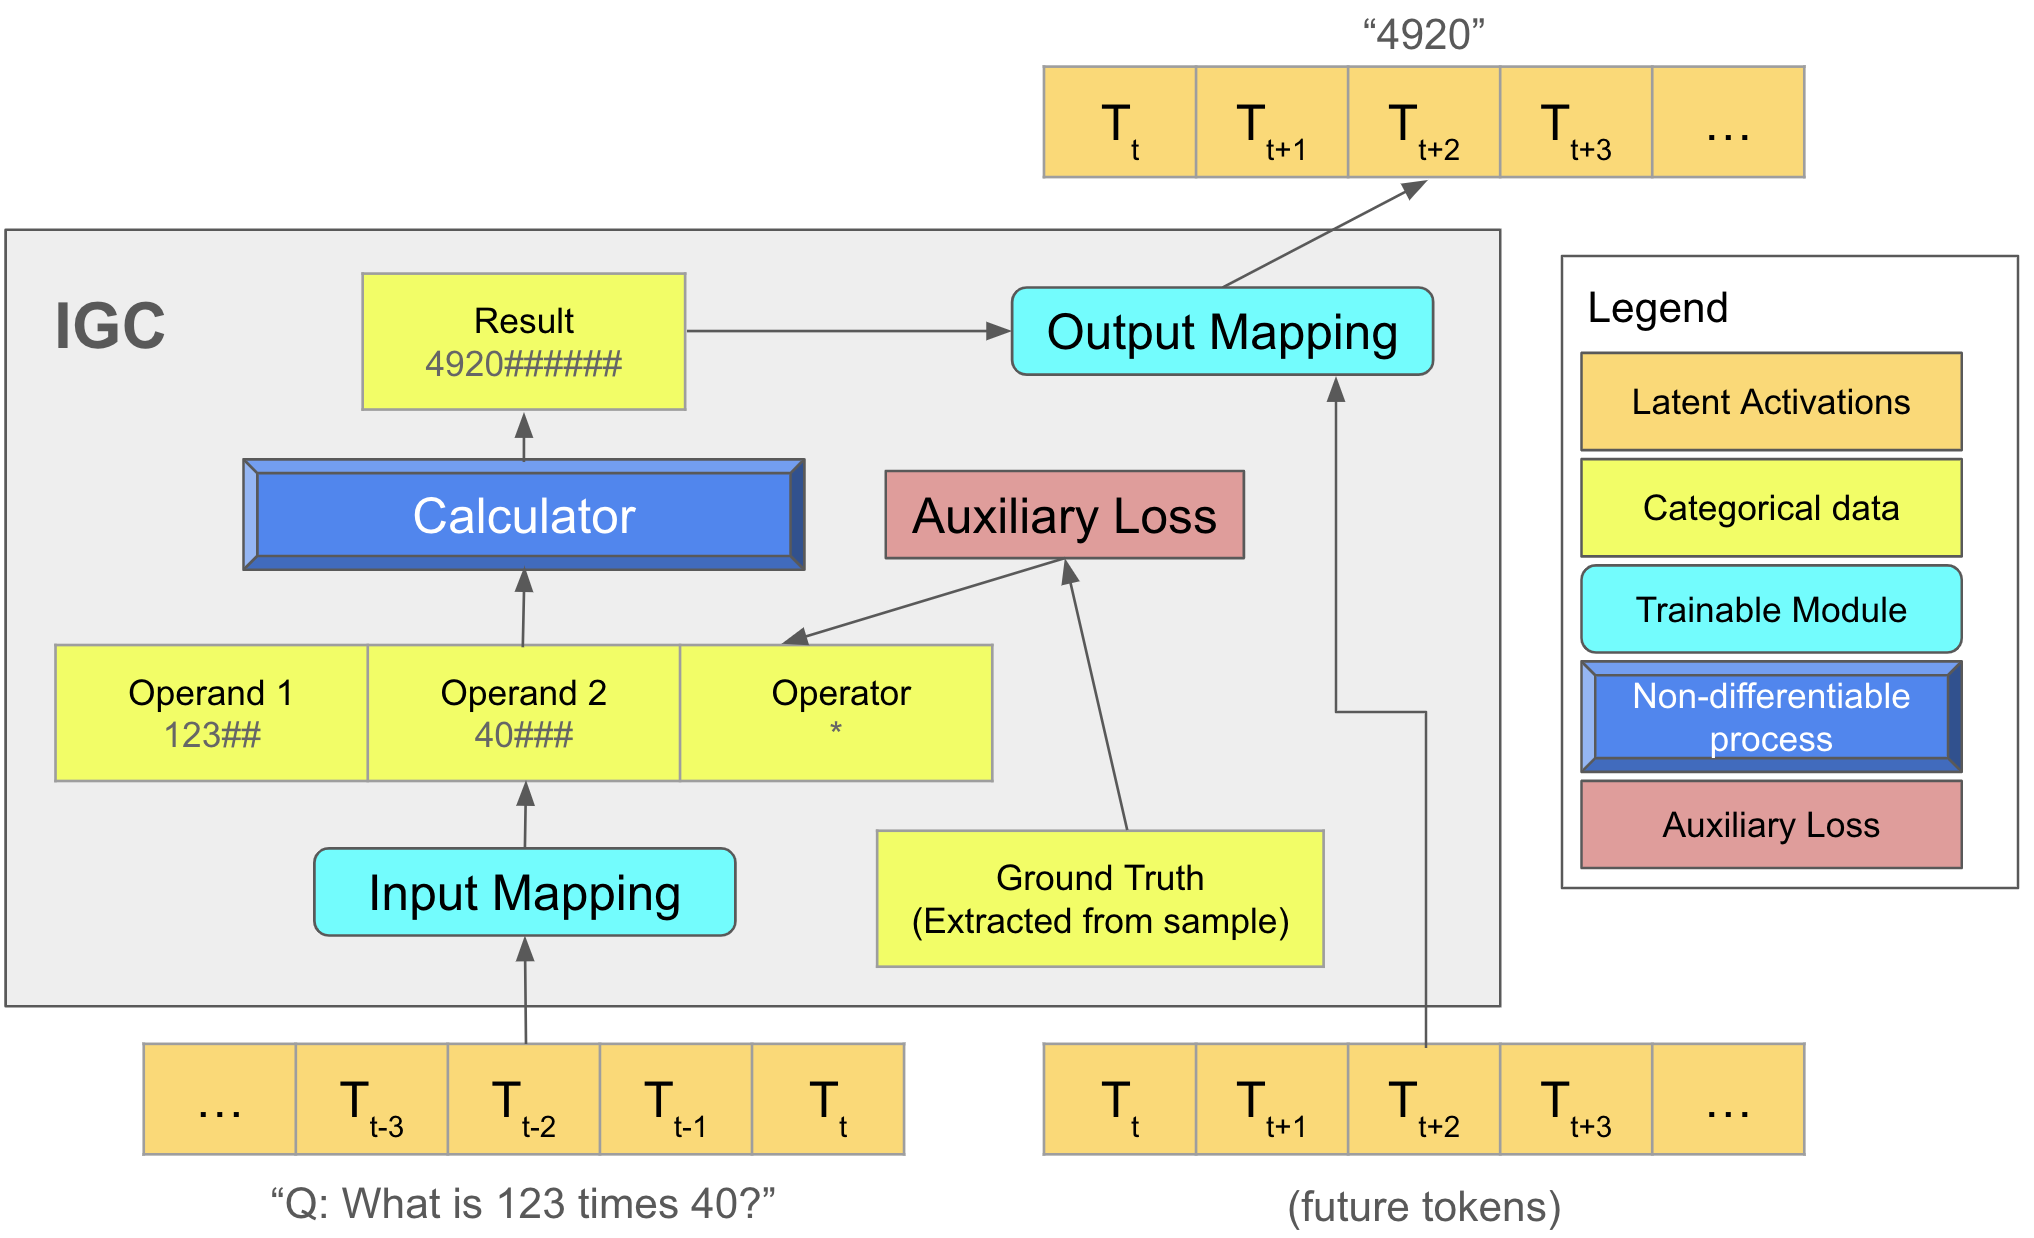
\includegraphics[width=0.714\linewidth]{images/architecture-summary.png}}
    \caption{
    % LEFT
    \textbf{Left}. The IGC is inserted into a pretrained LLM after a fixed layer, in this case layer 1. It modifies the output produced by that layer.
    % RIGHT
    \textbf{Right}. During training, the IGC takes the latent activations produced by the layer as its inputs and splits them into two parts: Before and after the anchor token $T_t$ at time step $t$, which has a special role for argument selection.
    % Three components
    The IGC comprises three components, two of which are trainable submodules:
    The Input Mapping submodule (Figure~\ref{fig:architecture-details}, left) uses the tokens before $T_t$ to extract the arithmetic task from the text and to format it for the calculator. It is trained through an auxiliary loss.
    The calculator itself is emulated on the GPU through a sequence of non-differentiable tensor operations. It is not a trainable component.
    The Output Mapping submodule (Figure~\ref{fig:architecture-details}, right) uses the results of the calculator to modify the tokens after $T_t$. It is trained by the LLM's normal loss function.
    % Inference
    Note that this image shows the training process using teacher forcing. During inference, the Input Mapping and the calculator are executed only on the iteration when the anchor token arrives. Their outputs are cached and reused on subsequent iterations.
    % OLD VERSION
    % It operates in three steps:
    % First, it extracts fixed-size, left-aligned inputs for the calculator from the variable-length inputs.
    % Second, it applies a non-differentiable operation that emulates a calculator and produces the output number in left-aligned digit format.
    % Third, it maps this number to all tokens produced at layer $n$ at time step $t$ and later, using trainable, dynamic gating weights.
    % Steps one and three involve trainable modules, but step two is non-differentiable. We therefore use an auxiliary loss to train the module of step one.
    % See Section~\ref{appendix-code} in the appendix for details.
    }
    \label{fig:architecture-main}
\end{figure*}


\begin{figure*}[t]
    \centering
    \frame{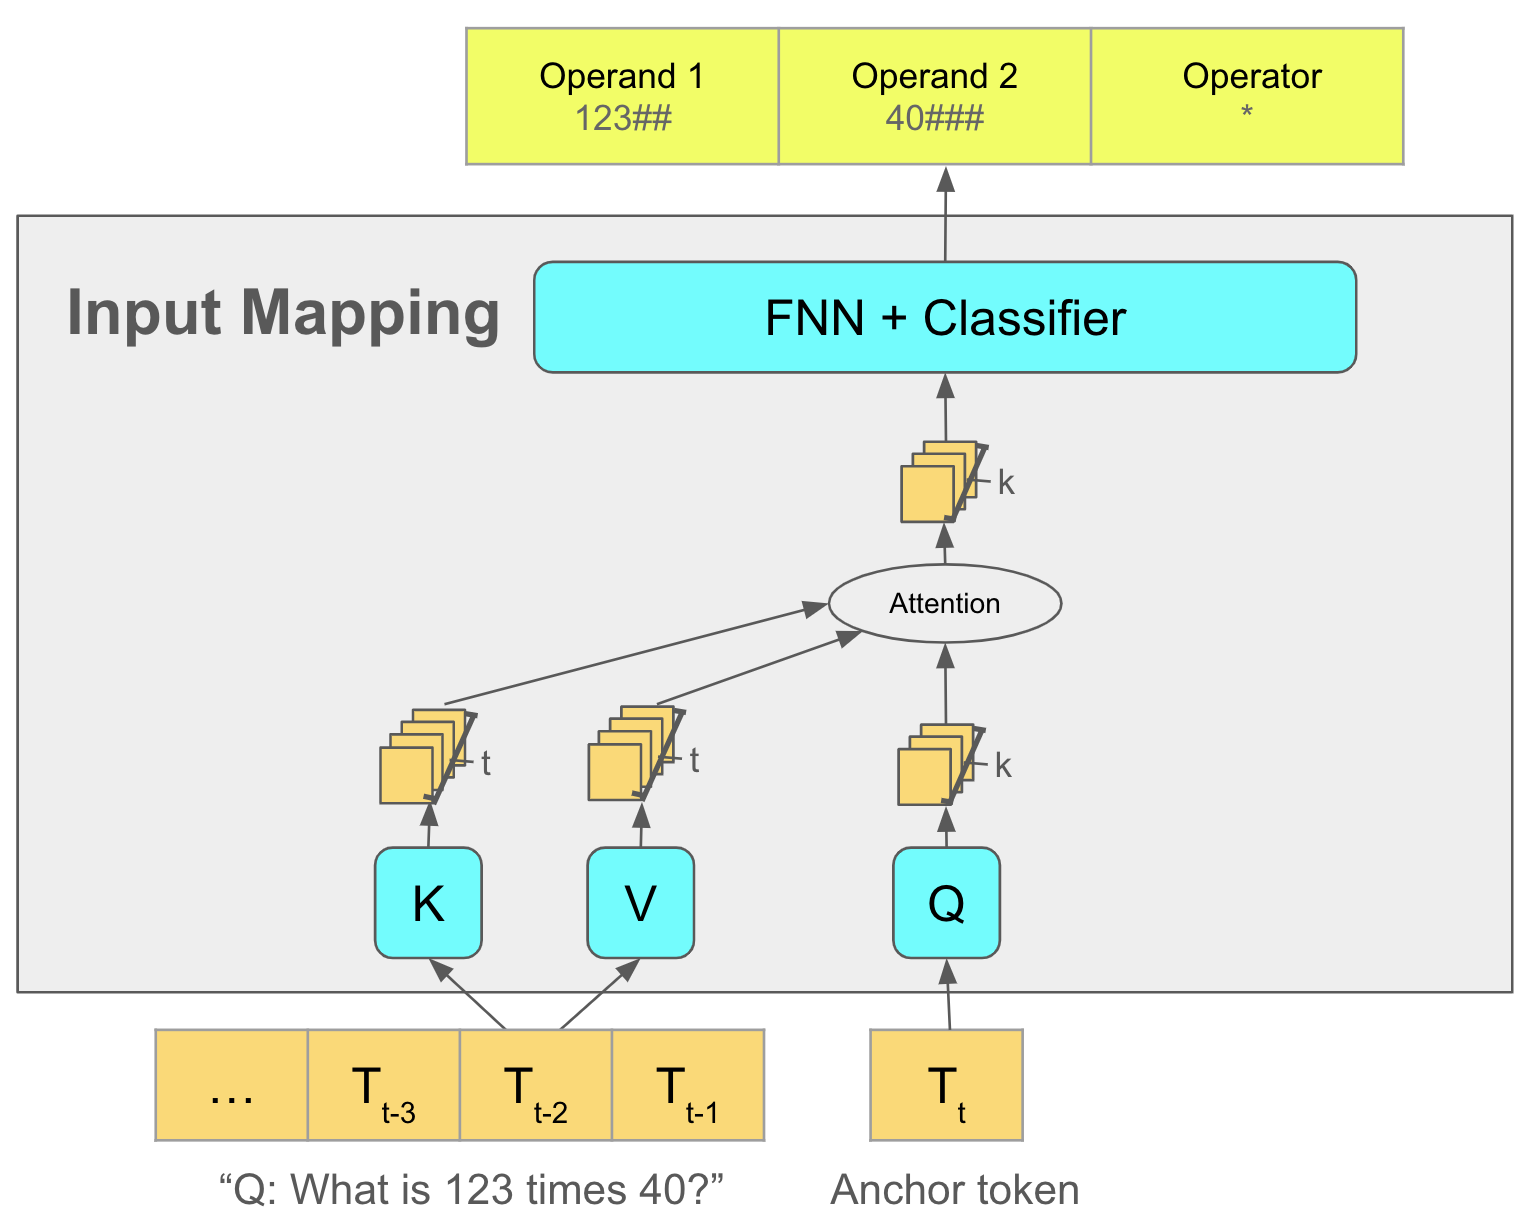
\includegraphics[width=0.497\linewidth]{images/architecture-input.png}}
    \frame{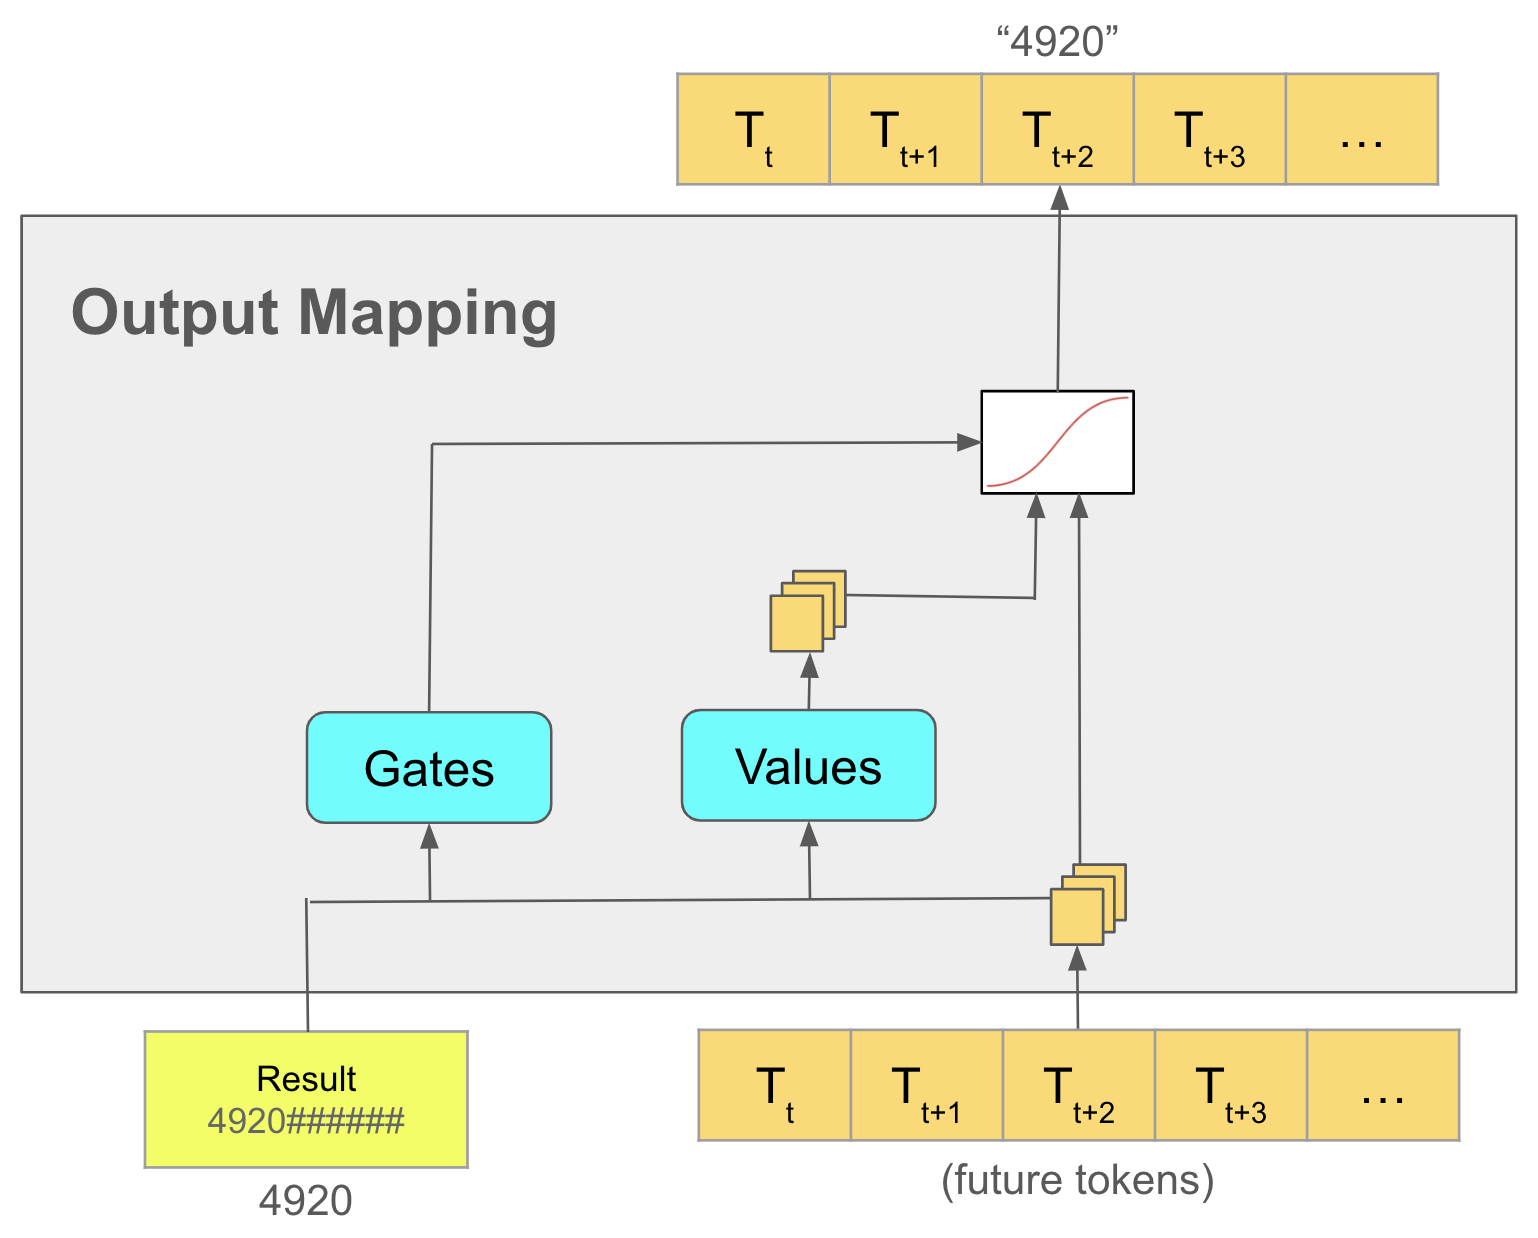
\includegraphics[width=0.496\linewidth]{images/architecture-output.png}}
    \caption{
    \textbf{Left}. The Input Mapping submodule takes variable-length textual embeddings and extracts the numbers and operator as fixed-length categorical data. The operands and operator are produced as probability distributions over possible digit values for each digit.
    \textbf{Calculator (not shown)}. The calculator discretizes the distributions produced by the Input Mapping submodule by sampling the most probable number and operator. It then emulates the arithmetic operation. The resulting number is formatted using one-hot encoding.
    \textbf{Right}. The Output Mapping submodule uses the fixed-length output of the calculator to modify each of the output tokens. This uses a separate learned gating weight for each token so that it can easily learn to leave tokens unchanged.
    }
    \label{fig:architecture-details}
\end{figure*}


\textbf{Approach}.
Figure~\ref{fig:architecture-main} gives an overview of our approach.
We introduce the Integrated Gated Calculator (IGC), a new module that modifies the output of an existing layer of a pretrained LLM.
We keep the LLM's existing weights frozen and train only the weights of the IGC.
% Similar to Adapter methods, but different
This is similar to Adapter-based tuning methods, but with several important differences:
\begin{itemize}
    \item It has non-differentiable components.
    \item It operates on multiple tokens at once.
    \item It is executed in discrete steps.
    \item It uses gated connections on its outputs.
\end{itemize}
We explain the reasons for and implications of each of these differences in the following.


\subsection{Main Considerations}


\textbf{Non-differentiable Components}.
The IGC uses tensor operations to emulate a calculator directly on the GPU.
The calculator's input and output digits are represented with discrete categorical data, which makes it a non-differentiable operation.
Therefore, the calculator itself is not a trainable component and it blocks the gradient coming from the LLM's main loss.
We therefore have two separate trainable components, which are illustrated in Figure~\ref{fig:architecture-details}: The Output Mapping, which is trained as normal, and the Input Mapping, which does not receive a gradient because of the calculator.
This necessitates a custom training method using an auxiliary loss, which we describe in Section~\ref{section-methods-training}.
% See Figure~\ref{fig:architecture-main} for the layout and Figure~\ref{fig:architecture-details} for details on the two submodules.


\textbf{Dependency on Multiple Tokens}.
% Last token is normally enough
Most applications of Adapter-based methods care about abstract concepts like sentiment, or about the presence or absence of specific named entities, since this type of information is often tested in Natural Language Benchmarks such as GLUE \citep{wang2019gluemultitaskbenchmarkanalysis,houlsby2019parameter}.
LLMs can encode such information in a single token or a fixed set of tokens.
However, numbers are encoded in several sequential tokens instead, and their relative position is crucial.
Our architecture needs to reflect this.
% We need variable-length encodings
We therefore have to learn a mapping from a variable-length set of tokens to the fixed-size input of the calculator.
Conversely, for the output, we need to map the fixed-size number back to all subsequent tokens.
We implement this through attention mechanisms and dynamic gating weights.
% No, really, this is necessary
We did try a simpler variant for comparison, in which the Input Mapping submodule used fixed inputs, and this architecture performed much worse.


\textbf{Discrete Execution}.
% Intuition
% NH: This doesn't read very well; don't use "second-person" rhetoric (a hypothetical "you"). I'm not even convinced the emphasising statements are needed, "is a discrete task" seems sufficient. --> I removed the second person. I think an explanation is needed because just saying discrete may not be clear for everyone.
Performing an arithmetic operation is a discrete task and not a distributed heuristic process. One does not perform $5\%$ of a calculation one moment and $\%7$ the next. A calculation is either performed or it is not. Our module is designed to reflect this:
% run only once
% NH: This is the only place PEFT is mentioned, do you really need the initialism? --> good catch! renamed it to adapter method. Same thing.
Most adapter methods work by applying a module to the \textit{current} token on \textit{each} iteration.
We instead perform no operations until we are sure that the arithmetic task has been fully described, at time $t$: When the chat switches from the user to the system.
The IGC is then run once, using all tokens available. The token $T_t$ at time $t$ is called the anchor token. The Input Mapping submodule uses it to construct a Query in an attention mechanism, to find all tokens relevant for the arithmetic operation.
% Difference between training and inference
During training, we use a form of teacher-forcing described in Section~\ref{section-methods-training}.
During inference, the results of our module at time $t$ are cached for later iterations.
% Why?
This unusual implementation has several benefits:
\begin{itemize}
    \item \textbf{More Effective Training}.
    We can not be certain what arithmetic operation is needed until all relevant tokens have been encountered. If we try to train the Input Mapping before all of the information it needs is available, it can only learn to guess. This would introduce noise and disrupt the training process.
    \item \textbf{Avoiding Redundancy}.
    If there is only one arithmetic operation, then every iteration after $t$ should learn to perform the exact same Input Mapping. There would be no benefit in repeating the operation multiple times.
    % \item \textbf{Efficiency}.
    % Since the module has to use all previous tokens as its input when it is called and affects all future tokens, training it is more expensive than traditional Adapter methods.
    % Calling it only once alleviates these issues and allows for a more efficient training process.
\end{itemize}


\textbf{Gated Outputs}.
The Output Mapping submodule uses gated connections with learned and dynamically calculated weights to modify the tokens after $T_t$.
It can learn how much each of the output tokens needs to be modified, and it can simply use near-zero weights to avoid making changes for tasks that do not require arithmetic.
% Benefit: No harmful side effects
As a consequence, the IGC causes no destructive interference in tasks where it is not needed.
We have experimentally confirmed that this works by testing our architecture on non-arithmetic tasks after training it for the arithmetic tasks described in Section~\ref{section-experiments}.
% OPTIONAL
These tasks used easily recognizable input templates, so confirming it for more complex word problems remains as future work.



\subsection{Training Method}
\label{section-methods-training}


Our training is based on the usual teacher-forcing approach. However, because the calculator is non-differentiable and blocks the gradient to the Input Mapping submodule, we have to slightly modify the algorithm.

\textbf{Ground Truth Data}.
We annotate our training data with ground truth data that specifies for each sample which arithmetic operation needs to be called, and with which operands.
% How realistic is it to have access to such helper data?
For simple arithmetic templates, this information can easily be extracted automatically.
% Future Work
For more difficult examples, such as word problems, training data can be created by the LLM itself, through a process analogous to the one described in the Toolformer paper \citep{schick2023toolformerlanguagemodelsteach}: The LLM annotates its existing training data with arithmetic operations that it believes would have been helpful. We then measure if annotating the data with the result of that operation reduces perplexity compared to the un-annotated data. If it does, we add the annotation to our training data.

\textbf{Modified Training Process}.
We use this helper information to modify the training process in two ways: Firstly, we apply an auxiliary loss to the Input Mapping component. This is just a simple cross-entropy loss that teaches the Input Mapping submodule to produce the correct input to the calculator. Secondly, we replace the output of the calculator with the correct output, so that the Output Mapping can begin training immediately, before the Input Mapping has converged. This second step is not strictly necessary, but speeds up training.

\textbf{One IGC execution per sample}.
In our training data, each sample requires exactly one use of the calculator, although these can happen at different times for each sample.
% Why? No reason not to. We explain later why it's helpful to have this limitation: It's clearer when to call the calculator and with what arguments.
This limitation simplifies the training process and allows for more efficient parallelization without loss of generality: Multi-step arithmetic tasks can simply be broken up into individual samples for each step of the calculation.



\subsection{Implementation Details}


\textbf{Effects of Tokenization}.
Previous studies have found that tokenization has a large impact on arithmetic abilities \citep{kim2021have,ding2022delta,liu2023goatfinetunedllamaoutperforms,tweet2024garrethlee}.
For training to be efficient, we need to ensure an inductive bias so that similar tokens can easily be mapped to similar internal representations, for both the input and the output of our module.
% Input and output of calculator need to be left-aligned.
% I.e., the most significant digit instead of the least significant digit is assigned to a fixed index.
The key consideration is that numbers are tokenized from left to right and the calculator's representation of digits must reflect this by being left-aligned: The most significant digit must be assigned to a fixed index, not the least significant one.
All architectures described in this paper use this left-aligned format.
% I'M SKIPPING EVERYTHING ABOUT THE TRAINING DATA.
% IT'S NOT INTUITIVE, AND I'M NOT 100% SURE MYSELF WHAT CAUSES THE BOOST IN PERFORMANCE.
% IT MIGHT JUST BE THAT A LARGER DATASET WOULD ALSO HAVE WORKED.
% % Dataset needs to be adjusted
% We can also use the tokenization method to generate more balanced datasets for training: By skipping samples whose token/position tuples appear frequently, we shrink our dataset, achieving both faster training speed and better generalization.
Additionally, we need to consider how digits are chunked into tokens.
While older versions of Llama used one token per digit \citep{yuan2023well,liu2023goatfinetunedllamaoutperforms}, Llama 3.1 \citep{dubey2024llama} groups numbers together in chunks of up to three digits.
This makes it harder for the model to infer the position of each digit, which caused significant problems when we used the more intuitive right-aligned format instead of the left-aligned one.
However, using the left-aligned pattern solved the problem and allowed us to meet and exceed the performance of other approaches.
We expect that the IGC can be adjusted to the tokenization methods and number representations used by other LLMs in a similar manner.
% See Appendix
See Section~\ref{section-tokenization} in the Appendix for details.
% Related paper / blog
% TODO check if this has been published / if he responded to my tweet
% https://x.com/garrethleee/status/1860039446311371132
% https://mail.google.com/mail/u/0/#inbox/KtbxLvHgPJCzTJgkNChjDfctBMPfKTvWGq
% This mirrors recent findings by \citet{tweet2024garrethlee}, who modified the tokenization of the same model we use as a basis and found that changing the tokenization to be right-to-left improves performance on arithmetic tasks.


\textbf{Choosing the Layer}.
We tried applying our module at several different layers of the LLM.
We obtained the best results at early layers.
% The hidden states are very similar to the tokens here, which makes both the input mapping and the output mapping easier to learn.
The results reported in our experiments are all based on applying the module to layer 1.
% We also tried reading from one layer and writing to another, but this performed poorly


% TODO OPTIONAL: mention the balanced training data here? Or elsewhere?




\section{Experiments}
\label{section-experiments}



\textbf{The BigBench Arithmetic Benchmark}.
In this paper we focus on arithmetic accuracy and not mathematical reasoning in general.
We therefore picked the BigBench Arithmetic benchmark for our evaluations \citep{srivastava2023beyond}.
It uses a deliberately simple template that focuses on raw arithmetic and has a good balance of different operators and input lengths.


\textbf{Alternate Templates}.
To ensure that the simplicity of the BigBench Arithmetic template does not skew results, we additionally trained and tested on several custom templates, as shown in Figure~\ref{fig:training_templates}, in order to make the task more diverse and challenging. We noticed no difference in performance between these templates.

% OPTIONAL: PUT THIS HERE OR IN FUTURE WORK, or skip it: It's a defensive explanation. Better to put it in a less important section of the paper.
% \textbf{Alternative Benchmarks}
% Mathematical datasets such as MATH \citep{hendrycksmath2021} and GSM8K \citep{cobbe2021gsm8k} are also popular, but would not be appropriate for our purposes: What makes them challenging is that the model has to determine the correct arithmetic operation to use from the text. However, the arithmetic operations themselves tend to be very simple.
% % MATH length distribution: [(1, 0.7097073180778974), (2, 0.8800642623220943), (3, 0.9580029247595312), (4, 0.9902370702972132), (5, 0.9939342135074458), (6, 0.9964367366274639), (7, 0.9980844884760355), (8, 0.9985685155815535), (9, 0.9992688101171964), (10, 0.9996086589359643), (11, 0.9997116434265), (12, 0.9997528372227142), (13, 0.9998661201623036), (14, 0.9998764186113571), (15, 0.9999176124075714), (17, 0.999927910856625), (18, 0.9999382093056786), (21, 1.0)]
% For example, in the MATH dataset, 70\% of numbers have only one digit, and 88\% have two digits or less.
% These datasets test mathematical reasoning ability, which is not the same as accuracy on arithmetic operations.

% To solve a math task effectively, an LLM needs to perform several steps: First it needs to extract the arithmetic operation(s) from the problem, then it needs to perform the arithmetic operation(s) correctly, and lastly it needs to format the output by turning it into a sentence.
% Of these three steps, only the second one is about solving arithmetic tasks.
% Finding the numbers to use from a word problem and formatting the output correctly are the responsibility of the base LLM, not of our module. They are therefore confounders for the purpose of evaluating arithmetic performance.
% Much of the difficulty of word problems stems from these steps that are irrelevant for evaluating raw arithmetic ability.
% word problems are full of confounders like these.
% Additionally, they often contain relatively short arithmetic tasks.
% To minimize the distracting impact of these confounders, we focus ...
% -
% “Word problems are also important, but out of scope”.
% -
% This paper is about finally finding a way to fix this elusive fundamental problem that arithmetic is hard. We make it possible to do arithmetic by adding a new building block into an LLM that does not rely on external tools and exists purely on the GPU.
% -
% Typical datasets for math that do involve text: GSM8K and MATH

% GOAT paper:
% They put a positive spin on using synthetic data only: “We systematically investigate the proposed decomposition method and demonstrate its effectiveness (Section 5). We conduct thorough experiments on the decomposition steps in a fully synthetic environment by mitigating many hard-to-control aspects of natural language. Our experimental setup offers an ideal platform to study the impact of CoT and intermediate supervision.“



\textbf{Comparisons}.
We modify a pretrained and instruction-finetuned Llama 3.1 8B model with an IGC, train it on synthetic data, and test it on the benchmark.
% Two sizes
The best existing results on the benchmark were achieved by PALM 535B \citep{chowdhery2023palm}, which is significantly larger than our model. We therefore also report the performance of relatively smaller models that are no more than one order of magnitude larger than our model.
% Can't make a good comparison
Unfortunately, a direct comparison with existing benchmark results is slightly unfair, since these were obtained with n-shot prompting instead of finetuning.
% Fairness by making it harder for ourselves
We deliberately make things harder for ourselves in order to strengthen the validity of our results: We report the \textit{average} performance of our runs and compare it to the \textit{best} performance of the n-shot runs.
% Finetuning baseline
Additionally, we also compare our model to a second baseline, which is based on finetuning: We enhance a Llama model with an Adapter method, using the same parameter count as our model, and finetune it on the same data.
% Comparisons aren't perfect, but doesn't matter
% It is unfortunately not possible for us to obtain benchmark results for a \textit{finetuned} version of PALM, but the quality of our results speaks for itself.
% Finetuning is better
It should also be noted that finetuning more accurately tests for arithmetic abilities than n-shot prompting does. This is evident from inspecting the benchmark results and comparing n-shot results for different values of $n$: There is a lot of variance in performance, even though the arithmetic tasks are exactly the same, and often the 1-shot version outperforms n-shot variants with higher $n$.
% OPTIONAL - unless I reference this again later, I could drop it
The loss of accuracy comes from an inability to understand the formatting required for the output, not an inability to perform the calculation.
% OPTIONAL, IF THIS IS CRITICIZED: Add comparisons to other papers that also used finetuning on BBA instead of n-shot prompting. Show that we are not the only ones.



\textbf{Results}.
Our model outperforms all baselines by a large margin.
\begin{itemize}
    \item Our model's performance is close to perfect across the board, even for the substantially harder subtask of multiplication.
    \item Our model is much better than the best of the smaller benchmark models.
    \item Compared to PALM 535B, which is optimized for mathematics and almost two orders of magnitude larger, our model is still slightly better for most subtasks and significantly better at multiplication.
    \item We significantly outperform our finetuning-based baseline, which shows that our model's great performance can be attributed to our novel architecture and not to the difference in evaluation methods.
    \item Our experiments had low variance and consistently converged to the reported values for multiple random seeds. In contrast, many of the n-shot benchmarks had high variance and the worst runs of our method still outperformed the best n-shot variants in the benchmark.
\end{itemize}

\textbf{Investigating Anomalies}.
% Anomaly 1
Curiously, our model performs slightly worse at the division subtask than the other operations, even though division is much simpler than multiplication. After investigating the possible causes, we attribute this to the fact that the BigBench Arithmetic benchmark used a different algorithm for generating random operands than we did. The test data therefore follows a different distribution than the training data.
% TODO OPTIONAL Is this worth reporting? Put a spin on it?
% Anomaly 2
% We also investigated why our finetuned baseline outperforms some of the weaker n-shot models: The Benchmark records show that many n-shot evaluations achieve less than $0.6$ accuracy even on 1-digit addition tasks. It is clear that the models can perform 1-digit addition, so this loss of performance comes from an inability to follow the formatting.



\begin{table*}
    \centering
    \begin{tabular}{|l|c|c|c|c|}
        \hline
        Task & Best small model & PALM 535B & Llama 8B baseline & IGC \\
        \hline
        \#Parameters & < 100B & 535B & 8B+17M & 8B+17M \\
        \hline
        Method & n-shot & n-shot & finetuning & finetuning \\
        \hline
        \hline
        \textbf{Overall} & 0.49 & 0.94 & 0.70 & \textbf{0.99} \\
        \hline
        Addition & 0.49 & 0.94 & 0.95 & \textbf{0.99} \\
        Subtraction & 0.69 & 0.96 & 0.88 & \textbf{0.99} \\
        Multiplication & 0.35 & 0.91 & 0.22 & \textbf{0.99} \\
        Division & 0.71 & 0.97 & 0.75 & \textbf{0.98} \\
        \hline
    \end{tabular}
    \caption{
    % TODO fix the footnote, it's not showing up.
    The accuracy of different models on the BigBench Arithmetic benchmark. The two columns about n-shot methods were extracted from official benchmark results, %\footnotemark,
    % \footnotetext{\url{https://github.com/google/BIG-bench/tree/main/bigbench/benchmark_tasks/arithmetic/results}}
    while the two finetuned variants were trained by us. We report the averages for the finetuned models and the best value for any $n$ for the n-shot benchmarks. Despite this lopsided comparison, our model still outperforms everything else.
    }
    \label{tab:performance_comparison}
\end{table*}



\textbf{Ablations}.
We also created hybrid modules in which the Input Mapping produces an additional output that is given to the Output Mapping submodule directly, making it end-to-end trainable just like a normal finetuning method.
% graph
Figure~\ref{fig:convergence-behavior} shows convergence behavior and final performance for several architectures: Our original IGC module without this shortcut, the IGC module with the shortcut, and a baseline that uses only the shortcut and uses no integrated calculator.
% OPTIONAL - explaining initialization may not be worth the space
% Initialization
All architectures start at zero accuracy because the LLM makes trivial formatting mistakes. They rapidly improve as they learn the template.
% Baseline
The variant that uses only the shortcut showed no improvements after this initial adaptation and its performance is equal to the finetuning baseline. This is unsurprising, since the pretraining likely already included basic arithmetic operations.
% Our module
The IGC module converges within 70 epochs and its test performance remains stable after convergence.
% Hybrid
We observe high variance in the test accuracy for the IGC+shortcut hybrid models, but their final performance is overall lower than the pure IGC without a shortcut connection.
We hypothesize that this is caused by overfitting and destructive interference: The finetuning component converges faster than the calculator, but it does not generalize well.

% In contrast, when not using finetuning but the calculator alone, there is no overfitting even over many epochs of training.
% in fact, there is some grokking: output-eval-bba continues to improve after output-eval-train has converged.
% (based on two measurements so far.)
% (Gather more data to check if this is consistently the case when using/not using finetuning components and for different training data).



\textbf{Model Sizes and Efficiency}.
% Llama
The IGC has 17 million parameters and is integrated into a pretrained Llama model with 8 billion parameters.
% PALM
Meanwhile, PALM 535B has almost two orders of magnitude more parameters than the Llama model, and four orders of magnitude more than the IGC.
% This is unoptimized
% It should be noted that we did not spend time optimizing our module's number of parameters either, so it is quite likely that our module could still work with even fewer parameters.
% Summary
The size of our module is trivial compared to the gain in performance it provides.
% This suggests that adding this module to an existing LLM during pretraining would be well worth it, even though arithmetic is only a specialized subtask.
% We describe in Future Work how this module could be integrated into an LLM during pretraining, which would likely be more efficient than the additive method we used in our experiments.
% Training time
The training process is fast and efficient as well: We generated an optimized dataset by filtering out frequently-occurring subsequences of tokens.
Using this technique, our models converged within two to four days of training with a set of only 10,000 samples, on a single GPU.
% Lastly, the additional time needed for running our model during inference is not noticeable / is smaller than random fluctuations between runs.
We note that such a small dataset is not enough for a normal model to learn how to generalize, as evidenced by our ablations.
This shows that our approach is less data hungry than alternative approaches.
We suspect that the reason for this is that the IGC's internal calculator is a perfect emulator, resulting in a much better inductive bias than a randomly initialized neural network.


\begin{figure}
    \centering
    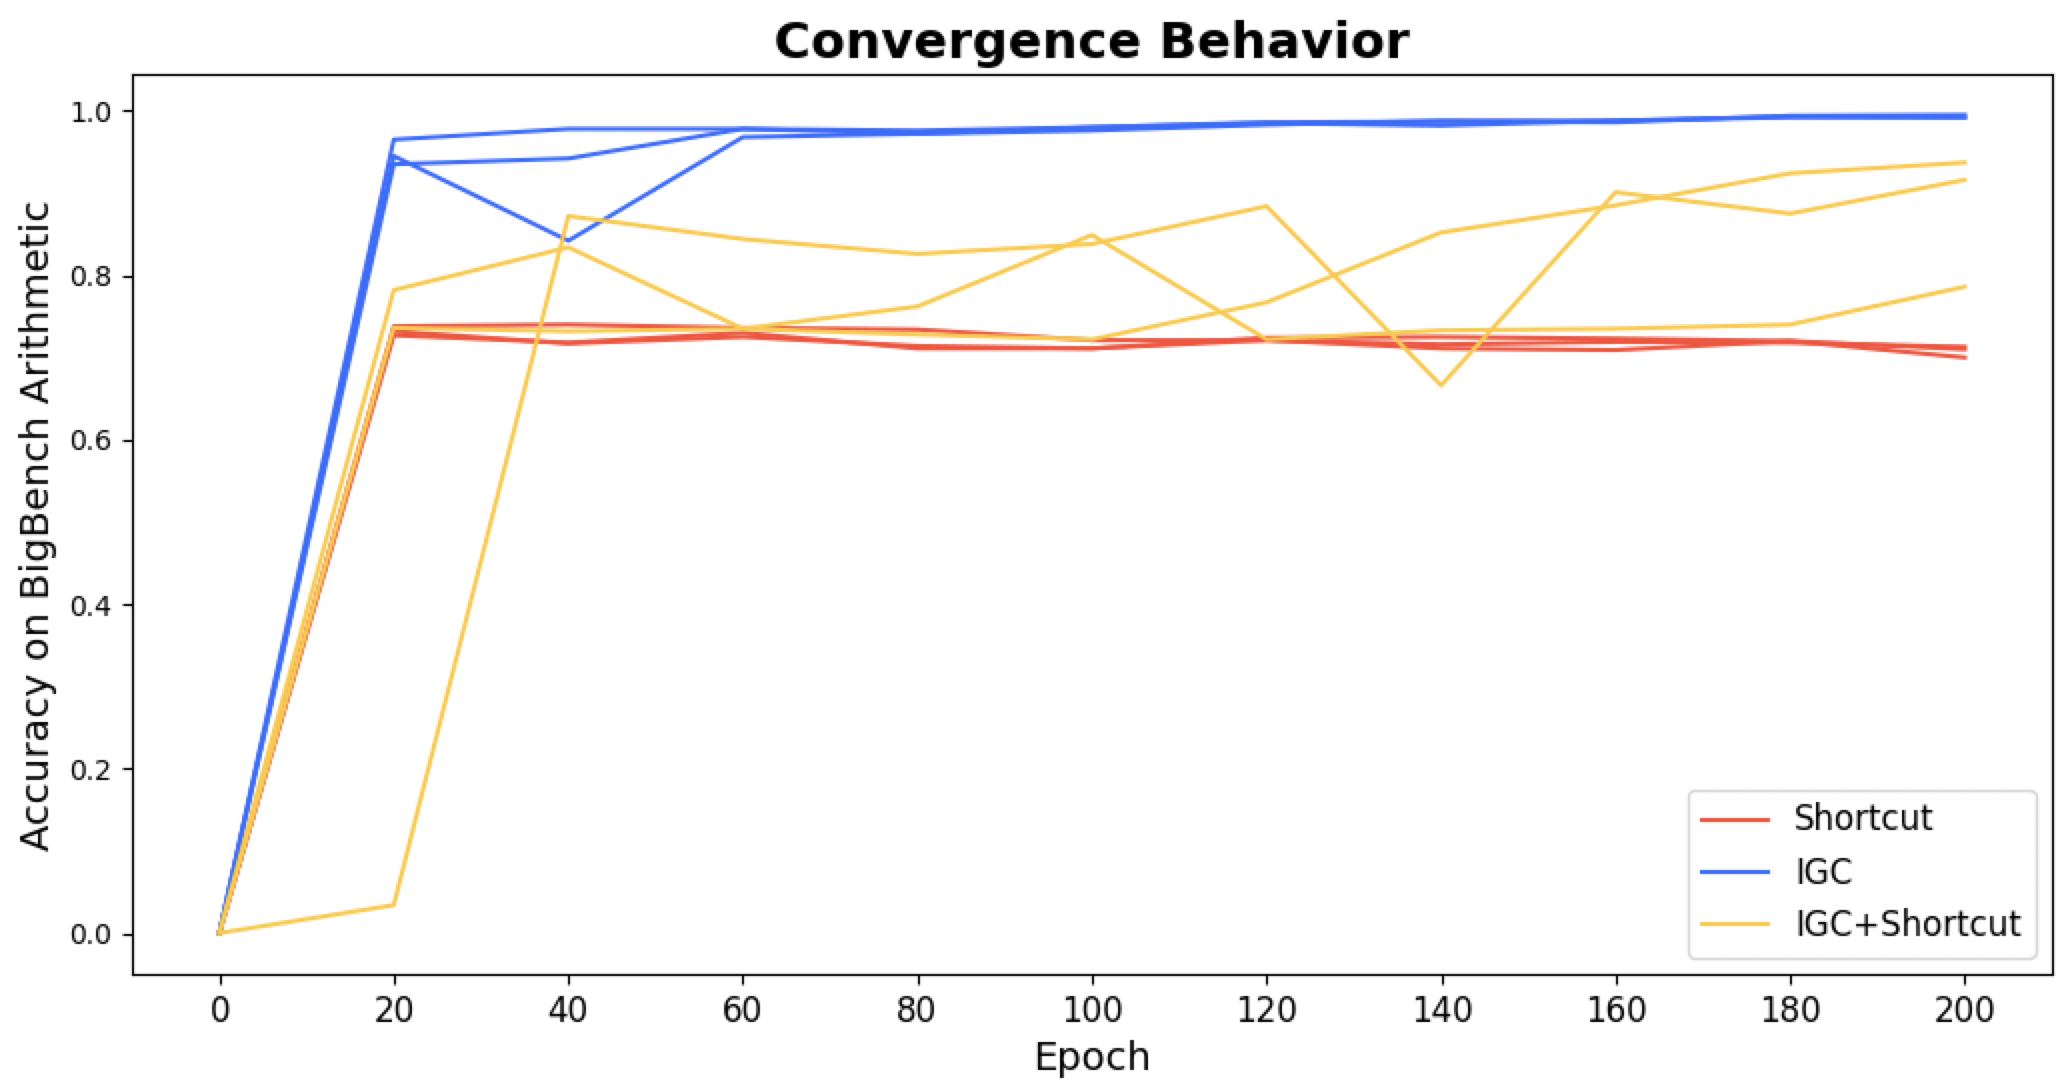
\includegraphics[width=0.95\linewidth]{images/convergence_behavior.png}
    \caption{
    The accuracy of various architectures on the BigBench Arithmetic benchmark as training proceeds.
    Multiple lines with the same color correspond to different random seeds for the same architecture.
    }
    \label{fig:convergence-behavior}
\end{figure}



\section{Comparison to Other Methods}
\label{section-comparison-of-methods}


Table~\ref{tab:comparison_of_traits} shows a high-level comparison between our method and other methods for solving arithmetic tasks.

\textbf{Capability}.
The only method that can solve arbitrary arithmetic tasks as reliably as the IGC is the use of external tools.

\textbf{Efficiency}.
Our method runs in a single step and avoids expensive transfers of data between GPU and CPU, making it more efficient than both COT and tool use.

\textbf{Interpretability}.
The IGC is highly interpretable because the numbers and operator are represented explicitly.
Moreover, the results of the calculation are mapped back to the LLM using learned gates, which allows us to measure how much they affect future tokens.

\textbf{Integration}.
We have reason to believe that our method can be more cleanly integrated into an LLM than other methods.
Firstly, the IGC is entirely \textit{internal} to the model and does not affect output tokens directly. This is important, because the output is an information bottleneck.
If the arithmetic operation is only a subtask of a larger task, needing to generate tokens for it may distract the LLM from its main task.
Additionally, teacher forcing generates separate gradients for each output token, which means that later steps taken for the same arithmetic operations can not repair mistakes made at earlier steps. In contrast, since the IGC is internal to the model and only executed once, it receives a single, coherent gradient.
% If basic arithmetic can be done implicitly, without requiring explicit thoughts (i.e. token outputs), then this should be helpful for thinking more efficiently because you don't get distracted.
Secondly, all three approaches (IGC, COT, tool use) share a common weakness, but only the IGC offers a path to fix that weakness:
All three approaches are \textit{added after pretraining}. This implies that the model can not know what the true result of a calculation is during pretraining. It is therefore forced to learn how to make plausible guesses.
Later, when we add the technique to solve arithmetic tasks correctly, the LLM has to unlearn these heuristics again.
% TODO OPTIONAL example
% Is the sum of two numbers prime?
% proof
The results of our ablation studies in Section~\ref{section-experiments} show that the presence of these incorrect heuristics is harmful and leads to a severe reduction in training speed and generalization ability.
% Fixing that with pretraining
Unlike COT and tool use methods, our method can be modified to avoid these problems:
We describe in Future Work how the IGC could be trained during pretraining (Section~\ref{section-future-work}).
% TODO OPTIONAL: toolformer paper acknowledges weakness:
% (however, later papers may have fixed that?)
% "One such limitation is the inability of Toolformer to use tools in a chain (i.e., using the output of one tool as an input for another tool). This is due to the fact that API calls for each tool are generated independently; as a consequence, there are no examples of chained tool use in the finetuning dataset. Our current approach also does not allow the LM to use a tool in an interactive way – especially for tools such as search engines, that could potentially return hundreds of different results, enabling a LM to browse through these results or to refine its search query in a similar spirit to Nakano et al. (2021) can be crucial for certain applications."

\textbf{Extensibility}.
Our method is specialized for arithmetic and trained on numbers up to a fixed length. By design, it can not help with any other type of task and it needs to be trained up to the largest number length we expect to see.
We address this in the Limitations (Section~\ref{section-limitations}) and explain why it is not much of a hindrance in practice.
We also note that the basic design of our module could be generalized and adjusted to other tasks. We describe how in Future Work (Section~\ref{section-future-work}).


\begin{table*}
    \centering
    \begin{tabular}{|l|l|c|c|c|c|}
        \hline
        \textbf{Feature} & \textbf{Feature Type} & \textbf{Basic LLM} & \textbf{COT} & \textbf{Tool use} & \textbf{IGC} \\
        \hline
        Addition \& Subtraction & Capability & \xmark & \cmark & \cmark & \cmark \\
        Multiplication \& Division & Capability & \xmark & \xmark & \cmark & \cmark \\
        \hline
        Single-step Solutions & Efficiency & \cmark & \xmark & \xmark & \cmark \\
        On GPU & Efficiency & \cmark & \cmark & \xmark & \cmark \\
        \hline
        Explicit Representations & Interpretability & \xmark & \cmark & \cmark & \cmark \\
        Modularity & Interpretability & \xmark & \pmark & \pmark & \cmark \\
        \hline
        Internal & Integration & \cmark & \xmark & \xmark & \cmark \\
        Pretraining & Integration & \cmark & \xmark & \xmark & \cmark \\
        \hline
        Dynamic Number Lengths & Extensibility & \cmark & \cmark & \cmark & \xmark \\
        Generically Extensible & Extensibility & \cmark & \cmark & \cmark & \pmark \\
        \hline
    \end{tabular}
    \caption{
    A comparison of different methods for solving arithmetic tasks.
    \textbf{Addition \& Subtraction}. Can the model generalize on addition and subtraction tasks?
    \textbf{Multiplication \& Division}. Can the model generalize on multiplication and division tasks?
    \textbf{Single-step Solutions}. Does the model run in constant time?
    \textbf{On GPU}. Does the model run entirely on the GPU?
    \textbf{Explicit Representation}. Can you tell when the model performs an arithmetic operation?
    \textbf{Modularity}. Can you tell how the model uses the results of an arithmetic operation?
    \textbf{Internal}. Is the arithmetic task solved entirely within latent variables, or does it need to generate output tokens?
    \textbf{Pretraining}. Is it possible to train the technique during pretraining, or is it only added afterwards?
    \textbf{Dynamic Number Lengths}. Can the model work with inputs of any size?
    \textbf{Generically Extensible}. Can the technique be extended to other tasks?
    }
    \label{tab:comparison_of_traits}
\end{table*}



\section{Future Work}
\label{section-future-work}



\textbf{Using the IGC during Pretraining}.
As explained in Section~\ref{section-comparison-of-methods}, it would be preferable if the IGC was trained directly during pretraining.
The difficulty here is that the IGC requires annotated training data for its auxiliary loss.
Fortunately, it should suffice to intersperse the LLM's normal training data with small amounts of our annotated arithmetic-specific data. During training, the IGC would be executed for all data, but its Input Mapping submodule would only be trained on this annotated data. For data that lacks this annotation, the submodule simply does not receive a gradient.
This makes the training process resilient to noise or even to mistakes in the remainder of the training data.
We note that it would be possible to apply the same technique to pretrain a tool-using model. However, doing so will increase the number of tokens produced for all affected samples, because the LLM needs to produce tokens in order to call tools. This reduces training efficiency and could even be actively harmful to performance because these additional tokens can act as a distractor. In contrast, since the IGC does not produce tokens and uses learned gates on its outputs, it is unlikely to cause any harm even when the dataset is annotated incorrectly.


\textbf{Word Problems}.
% Difference between word problem and arithmetic
Word problems are different from pure arithmetic problems: In addition to the ability to perform arithmetic operations, they also require the model to identify the correct operator and inputs from the text.
% Investigate integration into LLM
The IGC is only designed to perform arithmetic operations, so this is outside of its scope. However, it is relevant to investigate how effectively the IGC can be integrated into the LLM: When an LLM extracts an arithmetic task from a word problem, does it represent this task internally in a consistent manner, so that our Input Mapping submodule can access it effectively?
% Pretraining helps with integration
We expect that this integration will be better if the IGC is trained during pretraining: The Input Mapping submodule generates gradients that encourage the rest of the LLM to extract numbers in an interpretable format, but these gradients are ignored if we only train the IGC and keep the LLM's parameter's frozen.
% ----
% INTEGRATE THE BELOW WITH THE FRAMING: here are examples of word problems and here is why we did not do this already: It's out of scope and CONFLATES arithmetic with reasoning AND is actually worse at testing arithmetic
% ----
% OPTIONAL to mention this part
% \textbf{Alternative Benchmarks}
% Mathematical datasets such as MATH \citep{hendrycksmath2021} and GSM8K \citep{cobbe2021gsm8k} are also popular, but would not be appropriate for our purposes: What makes them challenging is that the model has to determine the correct arithmetic operation to use from the text. However, the arithmetic operations themselves tend to be very simple.
% % MATH length distribution: [(1, 0.7097073180778974), (2, 0.8800642623220943), (3, 0.9580029247595312), (4, 0.9902370702972132), (5, 0.9939342135074458), (6, 0.9964367366274639), (7, 0.9980844884760355), (8, 0.9985685155815535), (9, 0.9992688101171964), (10, 0.9996086589359643), (11, 0.9997116434265), (12, 0.9997528372227142), (13, 0.9998661201623036), (14, 0.9998764186113571), (15, 0.9999176124075714), (17, 0.999927910856625), (18, 0.9999382093056786), (21, 1.0)]
% For example, in the MATH dataset, 70\% of numbers have only one digit, and 88\% have two digits or less.
% These datasets test mathematical reasoning ability, which is not the same as accuracy on arithmetic operations.




% (OPTIONAL)
% TODO: Reread. Did I mention anything about multistep operations before? If so, I need to mention this here.
% \textbf{Multistep Arithmetic Reasoning}.
% this works much better if COT is used (https://arxiv.org/pdf/2210.09261) and performance is generally poor right now. Any improvement above random would be noteworthy. However, if the difficulty stems from chaining instead of from the difficulty of individual calculations, then having a calculator won't be very useful
% -
% currently it only runs once, at the anchor token
% -
% mention secondary training loss to later enable multi-step reasoning: only run when encountering the anchor token OR the previous iteration also used an IGC.
% -
% multiple calls. no calls. dependent call in multistep processes.



% (OPTIONAL)
% CIM, as a more generic version of the IGC
\textbf{Generalizing the IGC Mechanism}.
The core component of the IGC is a non-differentiable calculator. From the perspective of the trainable components, this is a blackbox.
That raises the question: What other mechanisms could be implemented in such a blackbox?
For example, if we replaced it with a lookup table and adjusted the training mechanism appropriately, it would enable the model to perform database lookups or knowledge graph traversals in a single iteration and without generating any tokens.
Such a mechanism could be used to improve upon the popular technique of Retrieval Augmented Generation \citep{lewis2020retrieval}.
% TODO (OPTIONAL)
% Also: Can combine multiple CIM as specialist modules, since each individual CIM/ has no side effect when its gating weights are set to zero



\section{Conclusion}


We introduce the Integrated Gated Calculator (IGC), a module that enhances an LLM with the ability to solve arithmetic tasks.
We achieve near-perfect generalization on the BigBench Arithmetic benchmark, outperforming all existing models.
In addition to its impressive performance, the IGC is also more practical than competing approaches: It avoids both the need for expensive tool calls, as well as lengthy and distracting Chains of Thought.
We discuss how to integrate our module into an LLM during pretraining and explain why this could improve the model's ability even further, supported by empirical evidence from our ablation studies.
Lastly, we note that our method could be generalized to integrate other types of non-differentiable tools into an LLM.





\section{Limitations}
\label{section-limitations}


\textbf{Fixed Maximum Length}.
By construction, the IGC uses a fixed maximum input length for its numbers. This size can be arbitrarily large, but can not be adjusted later.
To mitigate this issue, we can simply train the IGC with the largest size that we expect to see for the majority of practical tasks.
% Small numbers are normal
That number may be surprisingly small: In the MATH dataset \citep{hendrycksmath2021}, a standard benchmark for math word problems, 99\% of numbers have four digits or less.
% Approximate
In the rare cases when the model does have to deal with larger numbers, the LLM can still use the IGC as a very reliable approximator.
% External tools
It should also be noted that the IGC is not mutually exclusive with other methods: If the model encounters an arithmetic task that is both too large for the IGC \textit{and} that requires high accuracy, it can resort to calling external tools.
% Human-like
\textit{This mirrors human behavior}: We learn to solve numbers up to a certain size in our heads. If we encounter tasks more complex than that, we either perform a rough calculation, or we resort to tools.
Being able to solve simple arithmetic tasks in our heads without needing to use a tool is useful, but starting at a certain level of complexity it is no longer worth the effort.


\section{Acknowledgements}


This work was supported by a grant by the NHR Verein (National High Performance Computing, Germany).


\bibliography{main}



\appendix





\section{Tokenization}
\label{section-tokenization}


\textbf{The Problem}.
We experimented with different ways to construct the input and output format of our module to improve learning speed and generalization.
The basic goal is that similar tokens must be mapped to similar internal representations, for both the input and the output of our module.
The main hindrance to this is that tokenization groups multiple digits together into single tokens.


\textbf{Analysis}.
We have empirically analyzed the way tokenization works in our model:
Llama 3.1 8B uses a tokenization method that consistently parses numbers from left to right and groups digits together in groups of three, unless there are only two or one digit left. It also conveniently tokenizes in such a way that these 3-digit tokens do not contain non-numeric characters.
When read from the left, the tokens are always multiples of 3 digits, which makes it predictable which part of which token corresponds to which significant digit. For example, the 4th most significant digit always maps to the second token. Only the three least significant digits have any ambiguity.
In contrast, when you read from the right, then figuring out which token a digit belongs to depends on the length of the number, which is non-local information and therefore much harder to learn.
Table~\ref{tab:tokenization_examples} illustrates this.


% I'M SKIPPING EVERYTHING ABOUT THE TRAINING DATA.
% IT'S NOT INTUITIVE, AND I'M NOT 100% SURE MYSELF WHAT CAUSES THE BOOST IN PERFORMANCE.
% IT MIGHT JUST BE THAT A LARGER DATASET WOULD ALSO HAVE WORKED.
% \textbf{Consequences for the Training Data}.
% At first, we naively generated training data with random input numbers and operators.
% We analyzed the data generated in this manner and found that it generalized poorly because much of the training data was dominated by frequently occurring combinations of tokens and numbers.
% new training data leads to much faster training using less data, as well as improvements in accuracy
% -
% When training on an unbalanced dataset, the model is likely to learn simple but incorrect heuristics that happen to classify a lot of very similar datapoints correctly. In our-custom designed balanced dataset, it is much less likely for a simple heuristic to cover more than a small fraction of the data because there are no large clusters of similar datapoints.
% -
% We can also use the tokenization method to generate more balanced datasets for training: By skipping samples whose token/position tuples appear frequently, we shrink our dataset, achieving both faster training speed and better generalization.


\textbf{Consequences for the Architecture}.
The left-aligned format requires more work to implement because the position of the digit no longer matches the digit's significance.
Adjusting the architecture to work with left-aligned numbers requires two small changes:
% 11 options, placeholder
Firstly, each of the digits now needs to be represented as a classifier with eleven options instead of ten: One for each possible digits and one for the special placeholder symbol (an asterisk in Table~\ref{tab:tokenization_examples}).
% Shifting until the first placeholder
Secondly, extracting the number from a left-aligned representation requires an additional step compared to the right-aligned representation: We need to know the index of the first placeholder and shift the number accordingly to ensure we get the right magnitude.
% See code
This is demonstrated by the code in Section~\ref{appendix-code}.


\textbf{Results}.
We tried a right-aligned version of our architecture as well. The difference in performance was significant and in many cases the right-aligned variant failed to converge or to improve upon the performance of a finetuned model at all.


\textbf{Other Tokenization Methods}.
The left-aligned architecture described here works well because of the way Llama 3.1 tokenizes the data.
Other tokenization models may have different requirements and work better with other types of architectures.
We have written code to automatically analyze the distribution of tokens when generating training data. This code can help you to determine the optimal architecture to use. We will make it available upon acceptance of the paper.



\begin{table*}
    \centering
    \begin{tabular}{|l|l|r|l|}
        \hline
        Number & Tokenization & Right-aligned & Left-aligned \\
        \hline
        1234567890 & "123"456"789"0" & \texttt{\underline{123}456\underline{789}0} & \texttt{\underline{123}456\underline{789}0} \\
        123456789 & "123"456"789" & \texttt{0\underline{123}456\underline{789}} & \texttt{\underline{123}456\underline{789}*} \\
        12345678 & "123"456"78" & \texttt{00\underline{123}456\underline{78}} & \texttt{\underline{123}456\underline{78*}*} \\
        234567890 & "234"567"890" & \texttt{0\underline{234}567\underline{890}} & \texttt{\underline{234}567\underline{890}*} \\
        34567890 & "345"678"90" & \texttt{00\underline{345}678\underline{90}} & \texttt{\underline{345}678\underline{90*}*} \\
        \hline
    \end{tabular}
    \caption{
    Examples of numbers, how they get tokenized, and two different variants for representing them internally. Both variants use a fixed size of 10 digits for illustration. The right-aligned variant is the intuitive, default format, and puts the \emph{least} significant digit at a fixed index. In contrast, the left-aligned format puts the \emph{most} significant digit at a fixed index. The right-aligned format can be padded with zeros, but the left-aligned format requires a special symbol to mark where the number ends.
    The underlining in the two formatted numbers indicates which digits get grouped together into the same token. Note that the underlining is the same for all examples in the left-aligned format, but is inconsistent in the default format. This makes the mapping between the tokens and the format much easier to learn for the left-aligned format.
    The last two lines illustrates that removing digits from the left instead of the right as in the examples above does not lead to the reverse phenomenon: The tokenization is now different, so it doesn't help that the right-aligned representation is similar.
    }
    \label{tab:tokenization_examples}
\end{table*}


\section{Code}
\label{appendix-code}


% TODO
% adjust the code in the appendix to fully match the illustrations and text.
% Or make it clear that it's a simplified version and details are omitted?



In the following we provide python code for the three stages of our module.
% Note that these code snippets are incomplete and not optimized: They are intended to demonstrate how the module works in a readable way.


\subsection{Code of the Input Mapping and Auxiliary Loss}
\label{appendix-code-input-and-auxiliary-loss}


(We will provide code upon acceptance of the paper. The code in its current stage still needs to be optimized and documented for other researchers.)

% \begin{lstlisting}[language=Python]
% def perform_input_mapping_and_apply_auxiliary_loss(
%         hidden_states, anchor, input_mask, input_mapping_module, accumulator_for_additional_losses, calculator_input_target,
% ):
%     """
%     Extract a fixed-size encoding of data that the calculator can use from the variable-length network activations.
%     Also apply an auxiliary loss to the extracted values, since they will be used as input for the calculator, which is not differentiable.

%     :param hidden_states: The network activations after a specific layer of the LLM, including their positional encoding.
%     :param anchor: The token that corresponds to the last <|start_header_id|>.
%     :param input_mask: A mask with 1s up to the last <|start_header_id|> and 0s afterwards. This token represents the point where the calculator is called and may be different for each sample in the batch.
%     :param input_mapping_module: A module with several submodules, all of which can be simple and relatively small neural networks.
%     :param accumulator_for_additional_losses: A list of losses that will be added to by this function. At the end of the training step, the losses accumulated in here need to be added to the LLM's main loss before backpropagating.
%     :param calculator_input_target: The Operator, signs and left-aligned numbers used in this batch. This can be pre-calculated for each sample and passed along to the network during training. If the network is not being trained, this is None.
%     :return: The operator, signs and left-aligned numbers for the calculator to use.
%     """
%     batch_size, seq_length, block_size = hidden_states.shape
%     # The calculator requires a fixed number of tokens to work with.
%     # We arbitrarily pick 10 as the number of tokens we need because it is an upper bound:
%     # Each token encodes up to three digits, so we could represent two signed five-digit numbers
%     # and an operator with just 2*(2+1)+1=7 tokens.
%     number_of_required_tokens = 10
%     # Since the conversational history may contain more than one arithmetic operation,
%     # we need to anchor our query so that the module can learn to extract the correct set of tokens.
%     # For our purposes, a simple anchor that is based on the last <|start_header_id|> proved effective.
%     # Note that this may be insufficient for more complex usecases such as word problems.
%     # In these cases a multi-step mapping may be necessary to learn which of the tokens are relevant.
%     # Investigating this remains as Future Work.
%     composite_query = input_mapping_module.query_mapping(anchor)
%     query = einops.rearrange(composite_query, 'b (n l) -> b n l', n=number_of_required_tokens)
%     # Get a key for each hidden_state and match them to each of the queries,
%     # then apply a mask to prevent attending to the future.
%     key = input_mapping_module.key_mapping(hidden_states)
%     weights = key.bmm(query.transpose(1, 2))
%     assert weights.shape == (batch_size, seq_length, number_of_required_tokens)
%     assert input_mask.shape == (batch_size, seq_length, number_of_required_tokens)
%     weights = weights - (1 - input_mask) * 1e12
%     # Apply a regularization loss, not to be confused with the auxiliary training loss (!)
%     # It is an implementation detail that stabilizes convergence.
%     # It ensures that the values that get fed into the softmax are not too large, since this kills the gradient.
%     # This is necessary because the activation weights of a pretrained model are larger than
%     # those encountered in a randomly initialized model.
%     # After a few training steps, this quickly gets smoothed out
%     # and the regularization_loss becomes zero for the rest of training.
%     regularization_loss = nn.functional.mse_loss(weights, weights.clamp(min=-10, max=10).detach())
%     accumulator_for_additional_losses.append(regularization_loss)
%     # Apply the softmax after the regularization loss, then use it for attention over the hidden states
%     weights = weights.softmax(dim=1)
%     assert weights.shape == (batch_size, seq_length, number_of_required_tokens)
%     values = input_mapping_module.value_mapping(hidden_states)
%     assert values.shape == (batch_size, seq_length, 512)
%     inputs = weights.transpose(1, 2).bmm(values)
%     assert inputs.shape == (batch_size, number_of_required_tokens, 512)
%     inputs = einops.rearrange(inputs, 'b n l -> b (n l)')
%     # Now that we have extracted fixed-size information from the variable-length sequence of tokens,
%     # the next step is to derive a set of categorical variables for it.
%     calculator_input = input_mapping_module.fixed_position_tokens_to_categorical_values(inputs)
%     # There are two numbers of five digits and a sign each, plus the operator.
%     # To keep the code simpler each of these is represented as an 11-element categorical variable,
%     # although only the digits actually need that many options.
%     # (there are ten digits, plus a placeholder that is necessary for the left-aligned format to work.)
%     assert calculator_input.shape == (batch_size, ((5 + 1) * 2 + 1) * 11)
%     calculator_input = einops.rearrange(calculator_input, "b (k d) -> b d k", d=11)
%     assert calculator_input.shape == (batch_size, 11, 13)
%     # Calculate the auxiliary training loss, based on the ideal input of the calculator
%     if calculator_input_target is not None:
%         auxiliary_loss = nn.functional.cross_entropy(calculator_input, calculator_input_target)
%         accumulator_for_additional_losses.append(auxiliary_loss)
%     # Split the calculator_input into its components along the last dimension, so that the calculator can work with it
%     left_aligned_digits_of_both_numbers = calculator_input[:, :, :10].argmax(dim=1, keepdim=False)
%     input_number_signs = (calculator_input[:, 1, 10:12].gt(calculator_input[:, 0, 10:12])).long() * 2 - 1
%     tool_input_operator = calculator_input[:, :4, 12].argmax(dim=1)
%     return left_aligned_digits_of_both_numbers, input_number_signs, tool_input_operator
% \end{lstlisting}




\subsection{Code for Emulating a Calculator}
\label{appendix-code-emulator}



The calculator emulation works in three steps:
\begin{itemize}
    \item Translate left-aligned digits to numbers. We take inputs in a fixed-length categorical format that represents digits and translate this into a single number.
    \item Perform a calculation on the numbers. To ensure that the module can be trained on batches of data, we perform all four operations in parallel and then take a weighted average.
    \item Translate the result back into left-aligned digits.
\end{itemize}

\textbf{Numerical Accuracy}.
One important implementation detail to be aware of is the numerical accuracy of torch tensors. We only calculate up to 10 digits because that is all that is needed for the benchmark. If the calculator should be able to handle longer numbers that do not fit into a torch.int64 datatype, the calculation must be broken down into several smaller steps. This leads to code that is longer and harder to understand, although the operations are still fairly simple.

% \textbf{Optimization and readability}.
% Note that the below code is not optimized: It is fast enough, and more readable than optimized versions.
% The assert statements double as documentation: They indicate the shapes of the tensors.
(We will provide code upon acceptance of the paper. The code in its current stage still needs to be optimized and documented for other researchers.)

% TODO better formatting.
% tilde looks weird.
% .abs() is colored as a keyword even though it's a function.
% Maybe just make a screenshot of the code instead?

% \begin{lstlisting}[language=Python]
% def left_aligned_digits_to_number(digits, sign, max_length_of_number):
%     """
%     Convert a batch of left-aligned digits to the numbers they represent.
%     :param digits: A tensor with a categorical value, one per digit 0 to 9,
%     plus a placeholder, which is represented with the number 10.
%     :param sign: The sign of the number.
%     :param max_length_of_number: The number of digits.
%     :return: A tensor that contains the number represented by the digits.
%     """
%     batch_size = digits.shape[0]
%     assert digits.shape == (batch_size, max_length_of_number)
%     assert sign.shape == (batch_size,)
%     mask_for_placeholders = digits.eq(10)
%     digits_that_should_be_summed_up = digits * ~mask_for_placeholders
%     left_aligned_but_padded = torch.stack([
%         digits_that_should_be_summed_up[:, i] *
%         10 ** (max_length_of_number - i - 1)
%         for i in range(max_length_of_number)
%     ], dim=1).sum(dim=1) * sign
%     shift_by_placeholders = 10 ** mask_for_placeholders.sum(dim=1)
%     assert shift_by_placeholders.shape == (batch_size,)
%     result = left_aligned_but_padded // shift_by_placeholders
%     assert result.shape == (batch_size,)
%     return result

% def simulate_calculator(x, y, operator_idx):
%     """
%     Given a batch of number pairs and corresponding operators,
%     perform the correct calculation for each sample.
%     :param x: operand 1
%     :param y: operand 2
%     :param operator_idx: A categorical value that indicates the operation to use: 0=add, 1=subtract, 2=multiply, 3=divide
%     :return: The resulting number.
%     """
%     batch_size = x.shape[0]
%     assert x.shape == y.shape == operator_idx.shape == (batch_size,)
%     assert x.dtype is torch.int64 and y.dtype is torch.int64
%     plus = x + y
%     minus = x - y
%     mult = x * y
%     div = torch.full_like(x, fill_value=0.0)
%     div_mask = (y != 0)  # Avoid division by zero
%     div[div_mask] = x[div_mask] // y[div_mask]
%     ind_plus = operator_idx.eq(0)
%     ind_minus = operator_idx.eq(1)
%     ind_mult = operator_idx.eq(2)
%     ind_div = operator_idx.eq(3)
%     combined = ind_plus * plus + ind_minus * minus + ind_mult * mult + ind_div * div
%     assert combined.shape == (batch_size,)
%     assert combined.dtype is torch.int64, combined.dtype
%     return combined

% def number_to_left_aligned_digits(number, max_length_of_number):
%     """
%     Convert a batch of numbers to left-aligned digits.
%     :param number: A tensor containing an integer to convert.
%     :param max_length_of_number: The number of digits.
%     :return: A tensor containing the sign and a tensor with categorical values: The numbers 0 to 9, plus 10 as a placeholder.
%     """
%     batch_size = number.shape[0]
%     assert number.shape == (batch_size,)
%     sign = number.sign()
%     list_of_digit_tensors = [
%         ((number.abs() // (10 ** i)) % 10).long()
%         for i in range(max_length_of_number - 1, -1, -1)
%     ]
%     tmp = torch.stack(list_of_digit_tensors, dim=1)
%     non_zero_indices = tmp.ne(0).cumsum(dim=1).eq(0).sum(dim=1)
%     col_indices = torch.arange(tmp.shape[1], device=tmp.device).unsqueeze(0)
%     gather_indices = (col_indices + non_zero_indices.unsqueeze(1)) % tmp.shape[1]
%     gathered = tmp.gather(1, gather_indices)
%     mask = col_indices < (tmp.shape[1] - non_zero_indices.unsqueeze(1))
%     digits = gathered * mask + 10 * ~mask
%     assert digits.shape == (batch_size, max_length_of_number)
%     return sign, digits
% \end{lstlisting}


\subsection{Code of the Output Mapping}
\label{appendix-code-output}


% TODO

(We will provide code upon acceptance of the paper. The code in its current stage still needs to be optimized and documented for other researchers.)

% \begin{lstlisting}[language=Python]
% \end{lstlisting}



\end{document}
